%% technics.tex - Technics style LaTeX template. -*-Latex-*- %%%%%%%%%%%%
%%
%% (C) 2001 Joachim Nilsson <crash@vmlinux.org>
%%
%% This program can be redistributed and/or modified under the terms of
%% the LaTeX Project Public License. Available from the CTAN archives in
%% directory /macros/latex/base/lppl.txt; either version 1 of the 
%% License, or any later version.
%%
%%%%%%%%%%%%%%%%%%%%%%%%%%%%%%%%%%%%%%%%%%%%%%%%%%%%%%%%%%%%%%%%%%%%%%%%%

%
% \documentclass[12pt, twocolumn, twoside, draft]{article, report, letter, book}
\documentclass[12pt,twoside]{article}
\usepackage{technics}

\renewcommand{\companyname}{vmlinux.org}
\renewcommand{\companylogo}{vmlinux.eps}
\renewcommand{\doctitle}{\LaTeX\ Template for Technics Package}
\renewcommand{\preparedby}{Joachim Nilsson \url{crash@vmlinux.org}}
\renewcommand{\approvedby}{}
\renewcommand{\copyrightyear}{2001}


\title{\doctitle}
\author{\preparedby}

\begin{document}
\maketitle
\thispagestyle{fancy}
\tableofcontents

%\begin{abstract}
%\end{abstract}

%\cleardoublepage
\newpage
\section{Introduction}
The following two jobs are rolled into one with the modern WYSIWYG\footnote{What You See
Is What You Get} word processor.
You type your text, and as you go the text is given a concrete typographical
representation on the screen. Supposedly it corresponds closely to what you will
see when you send the same document to a printer, although for various reasons it
does not always do so. In effect, the text is continuously typeset as you key it
in. At first sight this may seem to be a great convenience; on closer inspection
it is a curse. There are three aspects to this.

\begin{enumerate}
        \item The author is distracted from the proper business of composing text,
        in favor of making typographical choices in relation to which she may have
        no expertise. ``Fiddling with fonts and margins'' when she should be
        focusing on content.

        \item The typesetting algorithm employed by WYSIWYG word processor sacrifices
        quality to the speed required for the setting and resetting of the user's
        input in real time. The final product is greatly inferior to that of a
        real typesetting program.

        \item The user of a word processor is under a strong temptation to lose
        sight of the logical structuration of the text and to conflate this with
        superficial typographical elements.
\end{enumerate}

\section{Rationale}
Writing business and technical documents requires the authors full attention to
be put on content rather than the above stated issues. \LaTeX\ offers an easy
way out of this trap. However, it is criticized for being to cryptic for day to
day work by computer illiterates. But do we really want the computer illiterates
to dictate the how we write our technical documents?

The obvious answer is an emphatic \emph{``No!''}. Still, any computer litterate
person needs the speed at which todays word processors operate without loosing
out to the poor quality those processors performs. To this end the Technics Package
was constructed. It provides an advanced typesetting of your technical documents
without your being aware of it.

\section{Usage}
This sample document serves as a template for all you wanting to use the
Technics package.

At the very end of this document, i.e., after the \verb+\end{document}+ tag, there
are examples of how to construct professional tables, include graphics as well as
adding a professionally typeset bibliography to your documents.


\section{Questions \&  Comments}
Questions and comments, even improvement patches (though probably not needed :-),
can be sent to the author at the below address:

\vspace{1.5cm}
\centering
Joachim Nilsson \url{<crash@vmlinux.org>}

%\subsection{Key bindings}
%\subsubsection{Key bindings -- WordStar}

\end{document}


%%%%%%%%%%%%%%%%%%%%%%%%%%%%%%%%%%%%%%%%%%%%%%%%%%%%%%%%%%%%%%%%%%%%%%%%%
%% To include a table with three columns complete with borders.
%% ``...in table~\ref{mytable} you can see an example of ...''
%%
%%%%%%%%%%%%%%%%%%%%%%%%%%%%%%%%%%%%%%%%%%%%%%%%%%%%%%%%%%%%%%%%%%%%%%%%%
%%\begin{table}[h]
%%\centering
%%\begin{tabular}{|l|c|l|}
%%\hline
%%\textbf{} & \textbf{} & \textbf{}  \\ \hline \hline
%%          &           &            \\ \hline
%%          &           &            \\ \hline
%%\textbf{} &           &            \\ \hline
%%\hline
%%\end{tabular}
%%\caption{}
%%\label{mytable}
%%\end{table}
%%%%%%%%%%%%%%%%%%%%%%%%%%%%%%%%%%%%%%%%%%%%%%%%%%%%%%%%%%%%%%%%%%%%%%%%%



%%%%%%%%%%%%%%%%%%%%%%%%%%%%%%%%%%%%%%%%%%%%%%%%%%%%%%%%%%%%%%%%%%%%%%%%%
%% To include a figure.
%% ``...in figure~\ref{lintel-logo} you can see an example of ...''
%% \begin{figure}
%% \includegraphics{graphics.eps}  % Don't forget to \usepackage{graphics}
%% \caption{A parody on Intel's logo.}
%% \label{lintel-logo}  % Order *IS* dependent, caption first and THEN label!
%% \end{figure}
%%
%% To reference the figure later (or earlier) in the document you use a
%% simple notation, like this: See figure~\ref{lintel-logo} ... 
%%
%%\bibliography{}             % Filename  of .bib-file.
%%\bibliographystyle{alpha}   % 
%%%%%%%%%%%%%%%%%%%%%%%%%%%%%%%%%%%%%%%%%%%%%%%%%%%%%%%%%%%%%%%%%%%%%%%%%

%%%%%%%%%%%%%%%%%%%%%%%%%%%%%%%%%%%%%%%%%%%%%%%%%%%%%%%%%%%%%%%%%%%%%%%%%
%% .bib-file sample:
%% @book{Lamport-94,
%%       author    = "Leslie Lamport",
%%       title     = "{{\LaTeX}: A Document Preparation System}",
%%       publisher = "Addison-Wesley",
%%       year      = 1994}
%%
%% Others: @article, @inproceedings, @techreport, ...
%% Example)
%%    Lamport \cite{Lamport-94} is a good book.
%% => Lamport [Lam94] is a good book.
%%
%% To generate:
%% 1. latex template.tex    => template.aux
%% 2. bibtex template.bib   => Generate references
%% 3. latex template.tex    => Includes references in template.aux
%% 4. latex template.tex    => Complete template.dvi
%% 5. xdvi template.dvi     => View result
%% 6. dvips template.dvi    => Printout to local printer.
%% 7. dvi2pdf template.dvi  => Generate Portable Document Format
%%
%% Steps 1->3 only neccesary if you have a separate BibTeX file.
%%
%%%%%%%%%%%%%%%%%%%%%%%%%%%%%%%%%%%%%%%%%%%%%%%%%%%%%%%%%%%%%%%%%%%%%%%%%



